\section{Introduction}
\label{intro}
Clean drinking water is the most valuable resource for humans. 71 percent surface of the world is covered with water but only 2.5 percent is considered fresh water. Any imbalance in water quality would seriously affect the health condition of humans. Now a day’s drinking water utilities are facing various challenges in real-time due to limited water resources, global warming, growing population, and pollution. Drinking water sources are also contaminated during frequent disasters such as floods, landslides, and cyclones. Hence there is a need for better methodologies for real-time water quality monitoring.
The UN and World Health Organization (WHO). Studies by WHO There are now 844 million people without a pure supplier of drinking water with a population of 159 million dependents on surface water. For pollution surface water can get contaminated by arsenic, various chemicals, imbalance of water quality parameter and micro bacteria. Unclean, potable water causes many diseases including diarrhoea, cholera, dysentery, typhoid and polio, which can result in life-threatening diseases. Even for contamination of water, the aquatic life gets a problem. Also, many people face these diseases every year in Bangladesh as well as other countries. This is estimated annually by the studies alarmingly. Recently, the challenges of water due to climate change, natural disaster, confined water, growing population, etc. have been encountered. However, the criteria of water quality must be seen in real time by higher methodologies in the future. Hence there is a need for better methodologies for real time water quality monitoring and controlling.


\section{Framework/Design Overview}
We developed a water quality monitoring and a controlling system where various physical and chemical sensors like pH sensor, turbidity sensor, flow sensor, ultrasonic sensor, waterproof temperature sensor are used. These sensors gather data from water and send data to Arduino UNO microcontroller. After internal data processing, Arduino sends data to NodeMCU and the wifi module sends these data to the google cloud server. we developed an android application to view these sensor data in real-time and it can download the previously stored data. Here is a cleaning brush that is used to clean the water tank and servo that opens the gate to flush the tank when water gets polluted and it sends an early alert by SMS to the owner with the tank location. Figure \ref{block} shows the block diagram of the proposed system.
\begin{figure}[h]
\centering
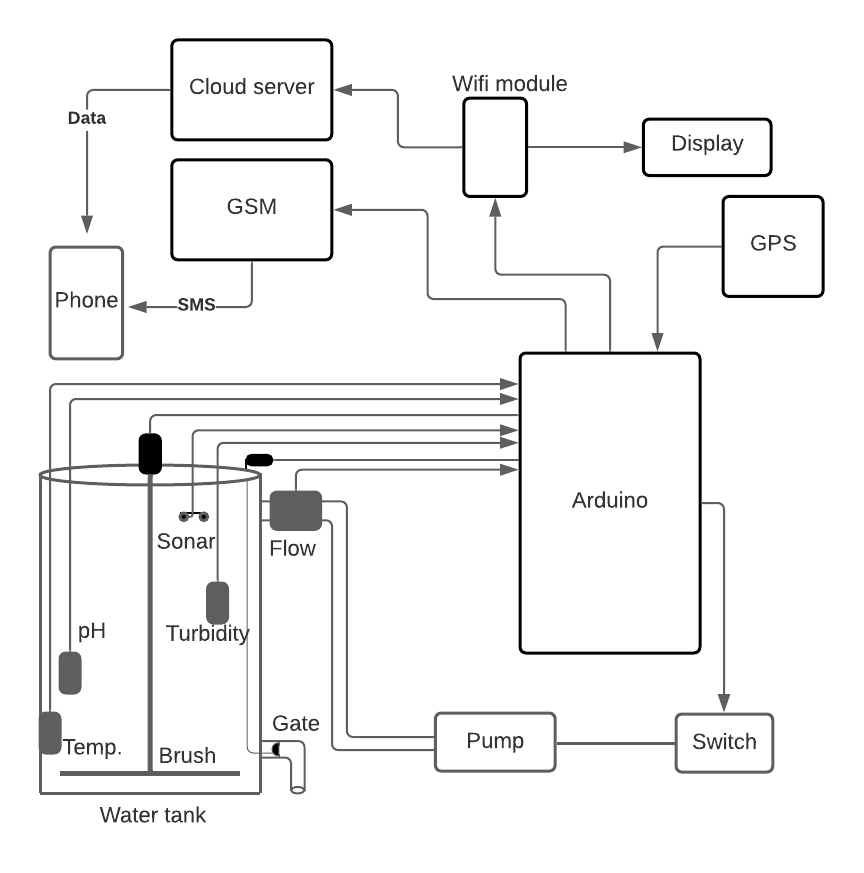
\includegraphics[width=1.0\textwidth]{figures/Block diagram.png}
\caption{Block diagram of the proposed system.}
\label{block}
\end{figure}


\section{Difficulties}
In this water project, various electronics are used. Many chemicals are dissolved in water at a tiny ratio. To calculates, the quantity of specific chemical perfectly is quite challenging. Water is harmful to electronics. Again any problem occurs in the mechanical component then the water will be licked. In this project NEO-6m GPS device is used which does not get location from satellite all the time. so at the time of sending a message to mobile phone if the location is unavailable then a message will be sent without location.  To send data to the cloud server continuous internet connection is needed and to run the whole system and continuous supply of electricity is needed. 
The following also several challenges:
\begin{itemize}
    
\item Higher quality sensor should be used otherwise the system will behave wrongly.
\item For flushing water higher quality non-return gate valve should be used otherwise it will not be able to capable of resisting high water pressure.
\item Keeping the whole system simple thus it can work perfectly.
\item Making the application interface user friendly.
\item It should be cost-effective.
\end{itemize}
\section{Applications}
This project can be used in many cases such as:
\begin{itemize}
\item Water quality monitoring and the controlling system can be used in urban and rural area water supply area. 
\item In agricultural and industrial applications, this system can also be introduced.
\item This project can also be used for treating water of WASA and home water tank.
\item This method can also be used for treating and managing wastewater before discharging it into a freshwater cell.
\item This method can also be used for aquaculture.

\end{itemize}

\section{Motivation}
Nowadays in city and village, people use the tank as a reservoir. Again day by day the surface water level is undergoing and the water layer gets damaged for many natural and man-made reason. For getting the very deep layer of water people depends on the supply of water. Those tanks are so big and placed at the top of the house or city. So generally for a long period tank does not get cleaned. So dissolved iron and dirt get dissipated at the bottom of the tank. So often WASA and home water tank supply dirty water. Again water is used continuously so generally tank does not make clean. Most people in urban use supply water for all the purposes, so unbalancing of water quality causes health problem and harmful for aquatic life. And people suffer from many diseases. Till this time many systems developed regarding monitoring the water quality but no system has a quality controlling feature. All those developed systems have many limitations. 

By observing those problems, we designed a water quality motoring and controlling system based on internet of things technology as IoT can make a system automated and faster \cite{gubbi2013internet} which can monitor water quality parameters and automatically clean tank when water gets unacceptable to use.

\vspace{1cm}


\begin{figure}[h]
\centering
\subfloat[Water tank]{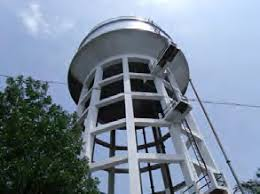
\includegraphics[width = 0.4\textwidth]{figures/tank1.jpg}} 
\hspace{1in}
\subfloat[Sample dirty water.]{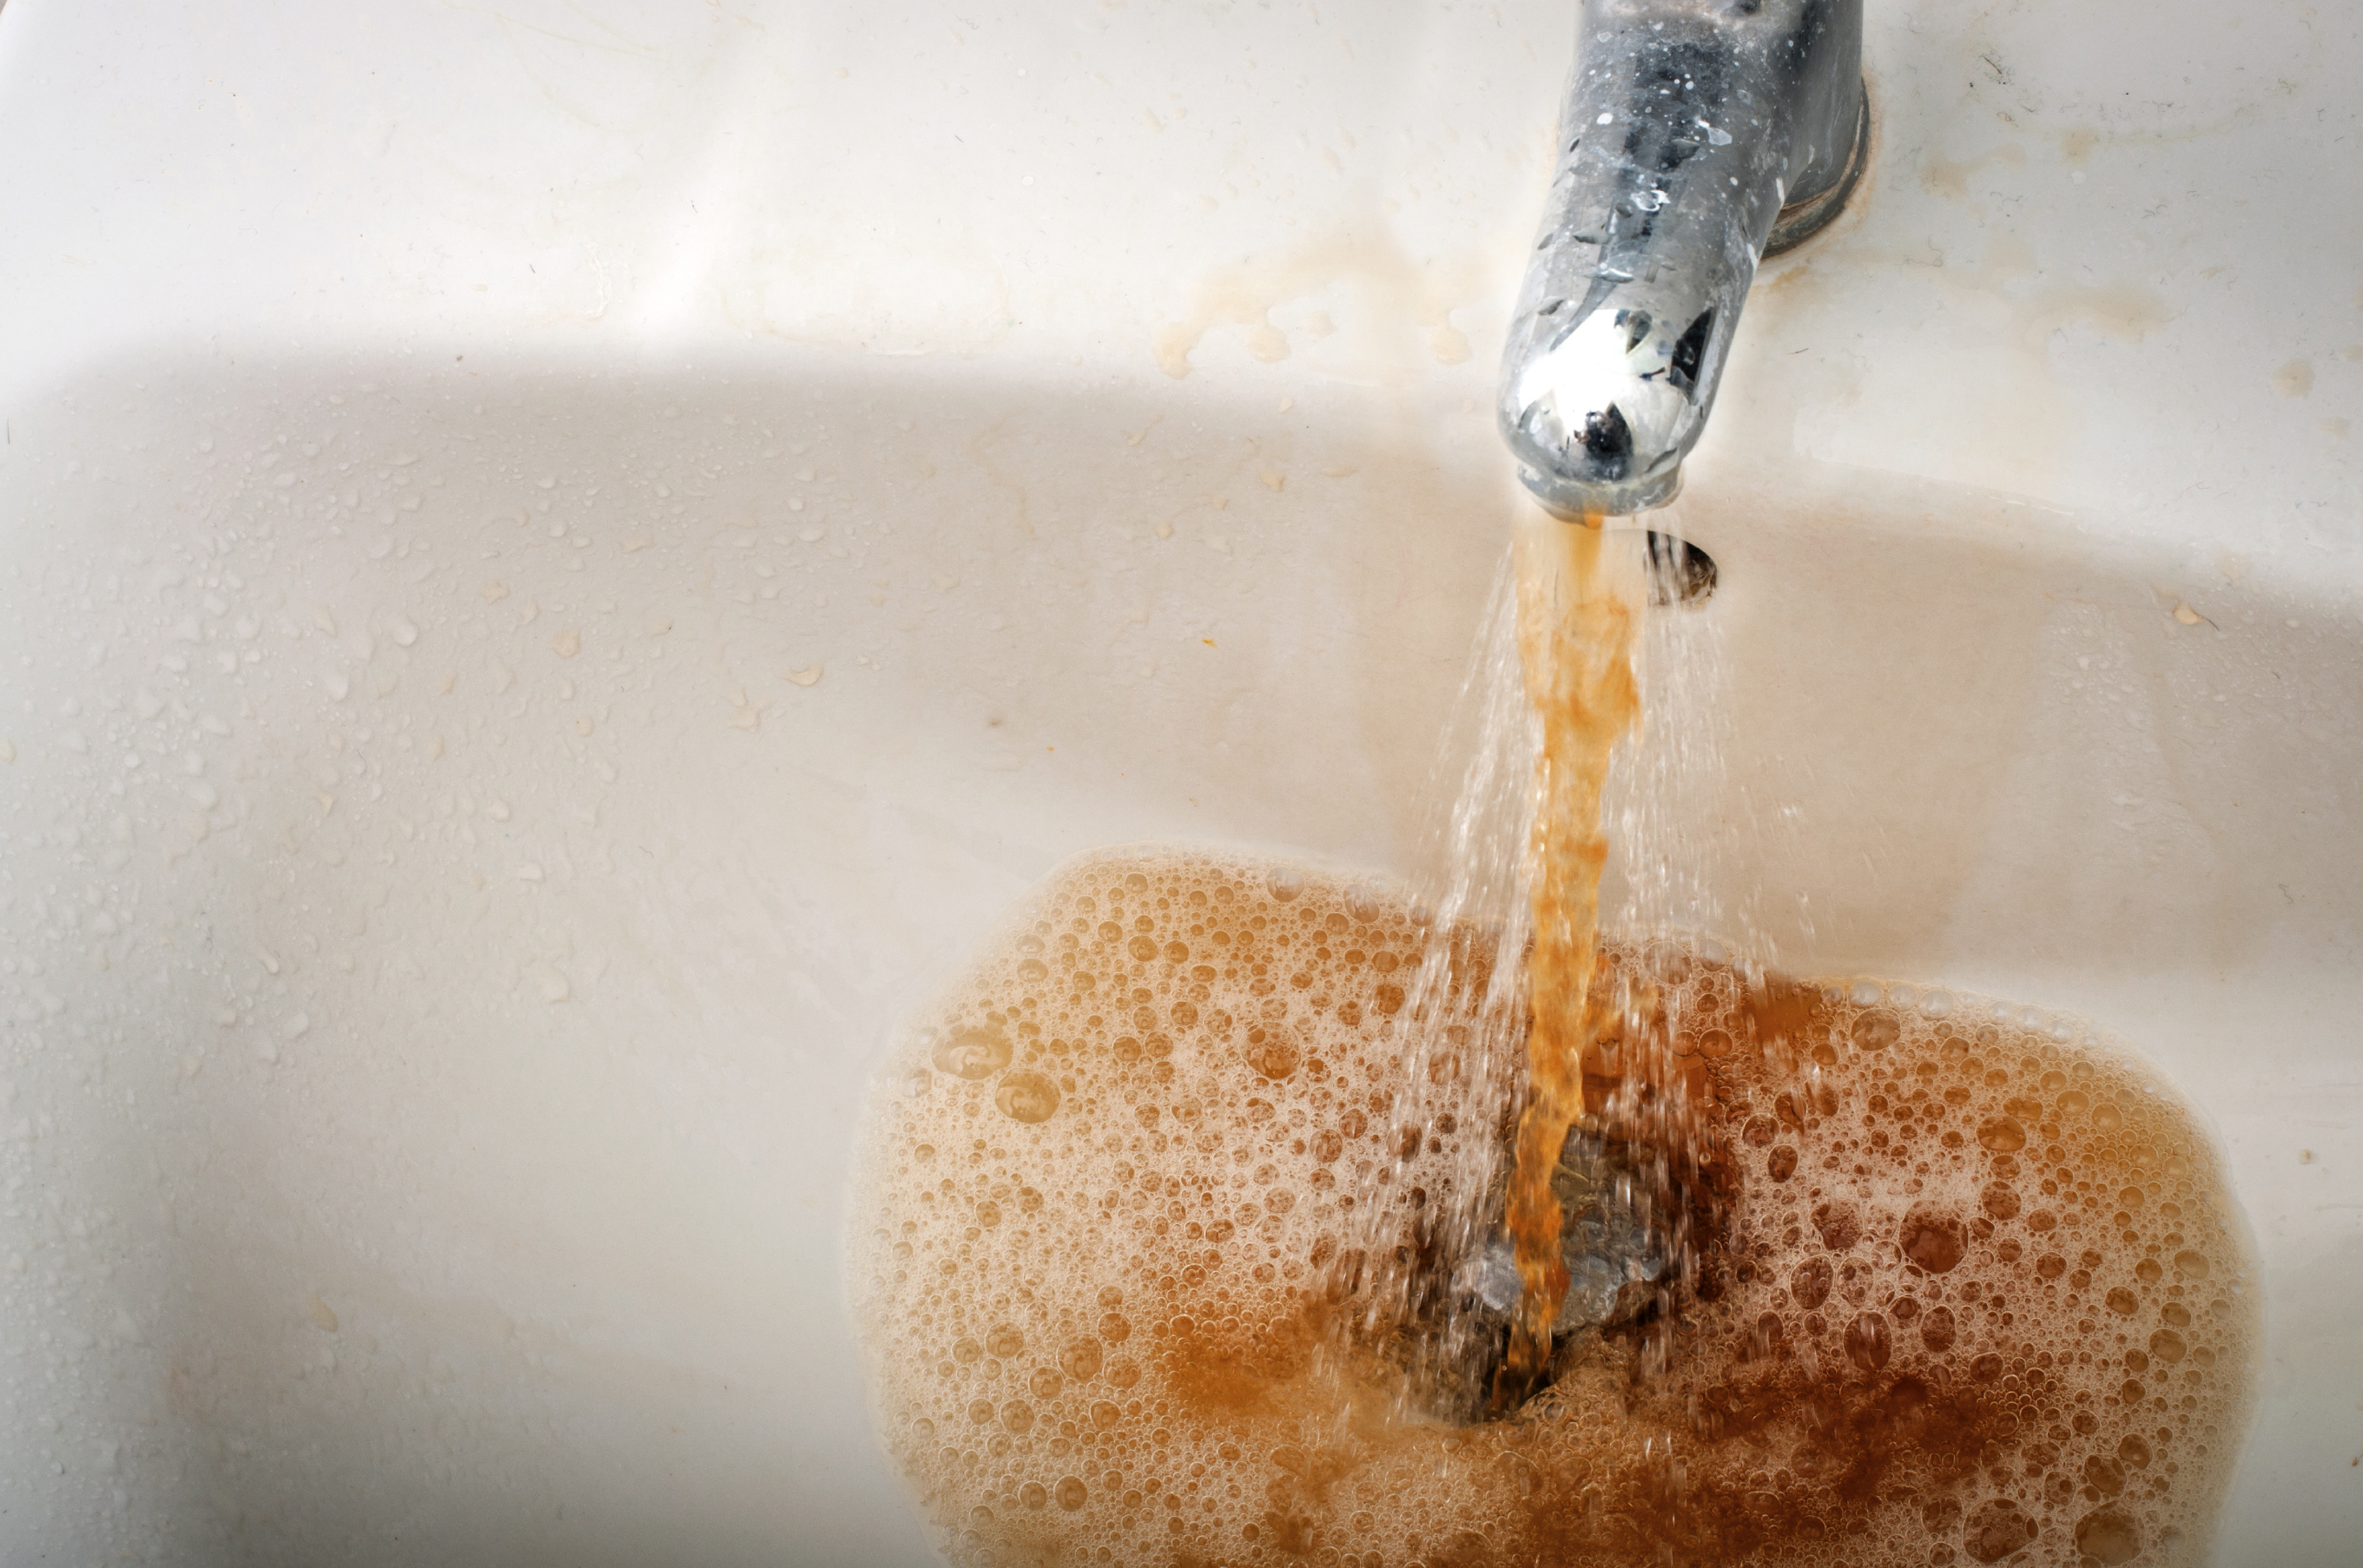
\includegraphics[width = 0.4\textwidth]{figures/dirty1.jpg}}

\caption{WASA water}
\end{figure}

% \begin{figure}[H]
% \centering
% 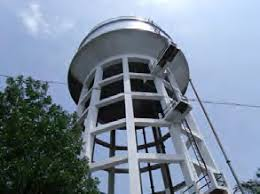
\includegraphics[width=0.6\textwidth]{figures/tank1.jpg}
% \caption{Water tank.}
% \label{sample}
% \end{figure}

% \begin{figure}[H]
% \centering
% 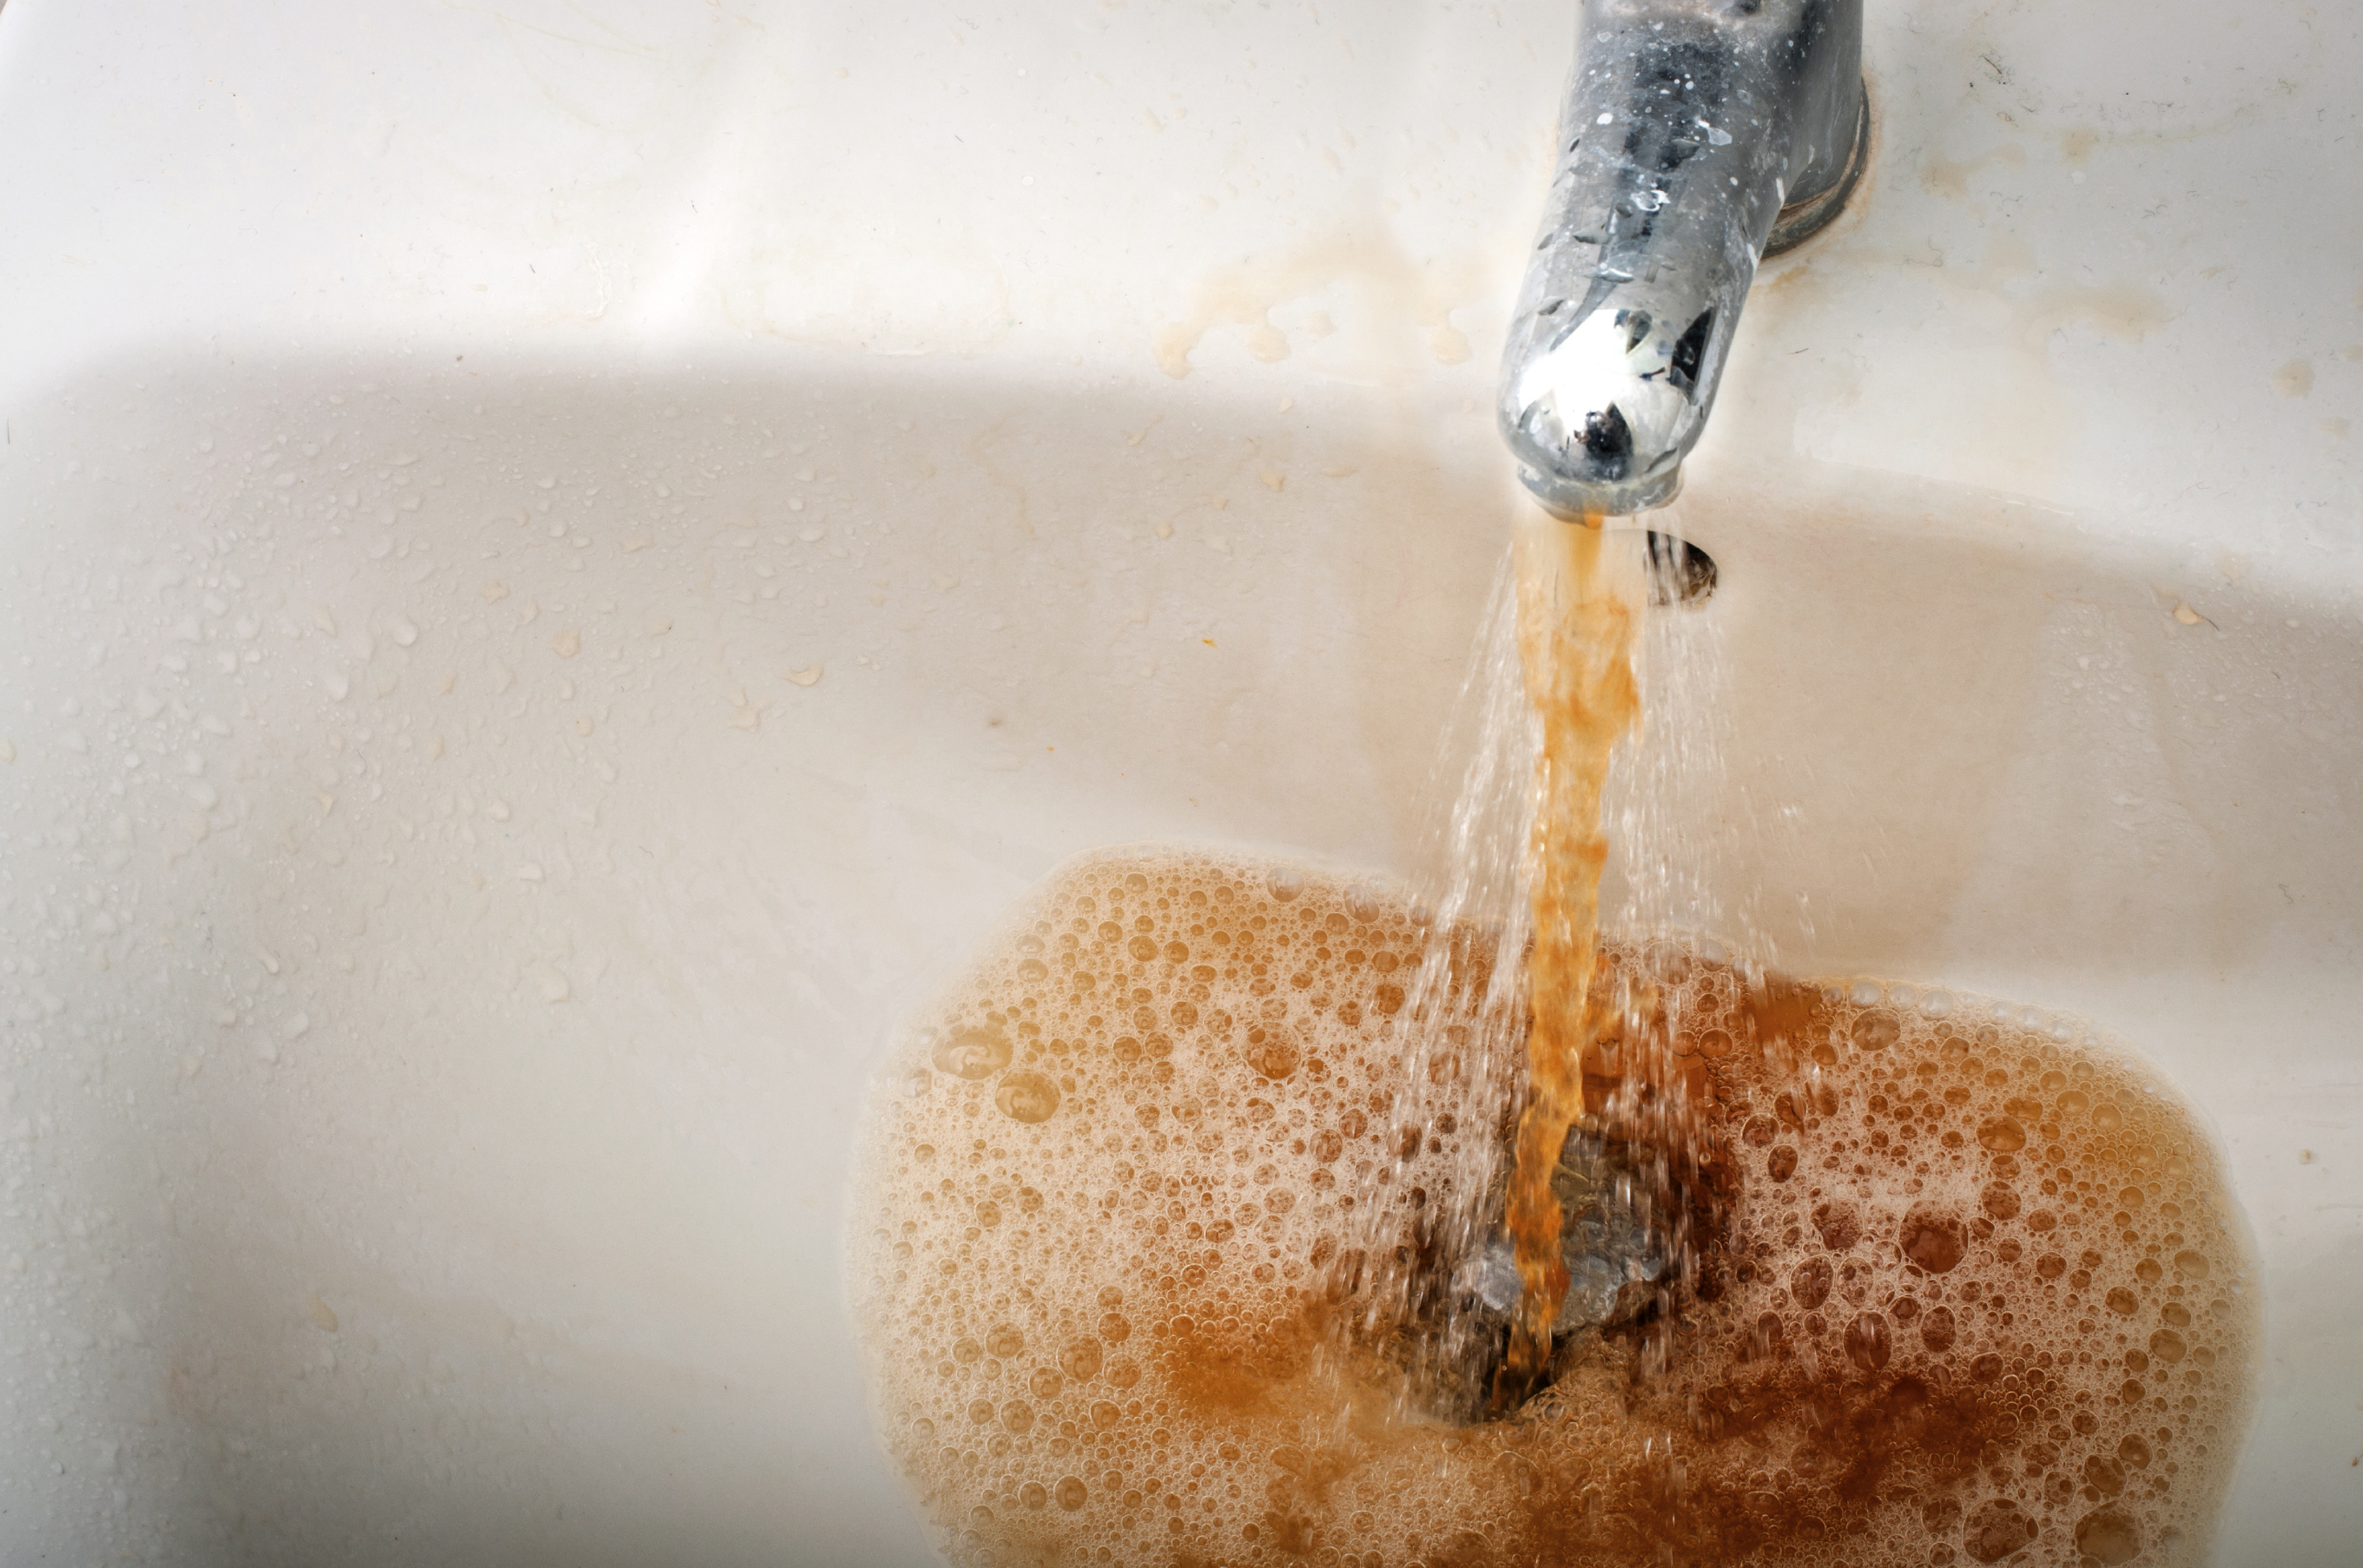
\includegraphics[width=0.6\textwidth]{figures/dirty1.jpg}
% \caption{Sample dirty water.}
% \label{sample}
% \end{figure}

% \begin{figure}[H]
% \centering
% 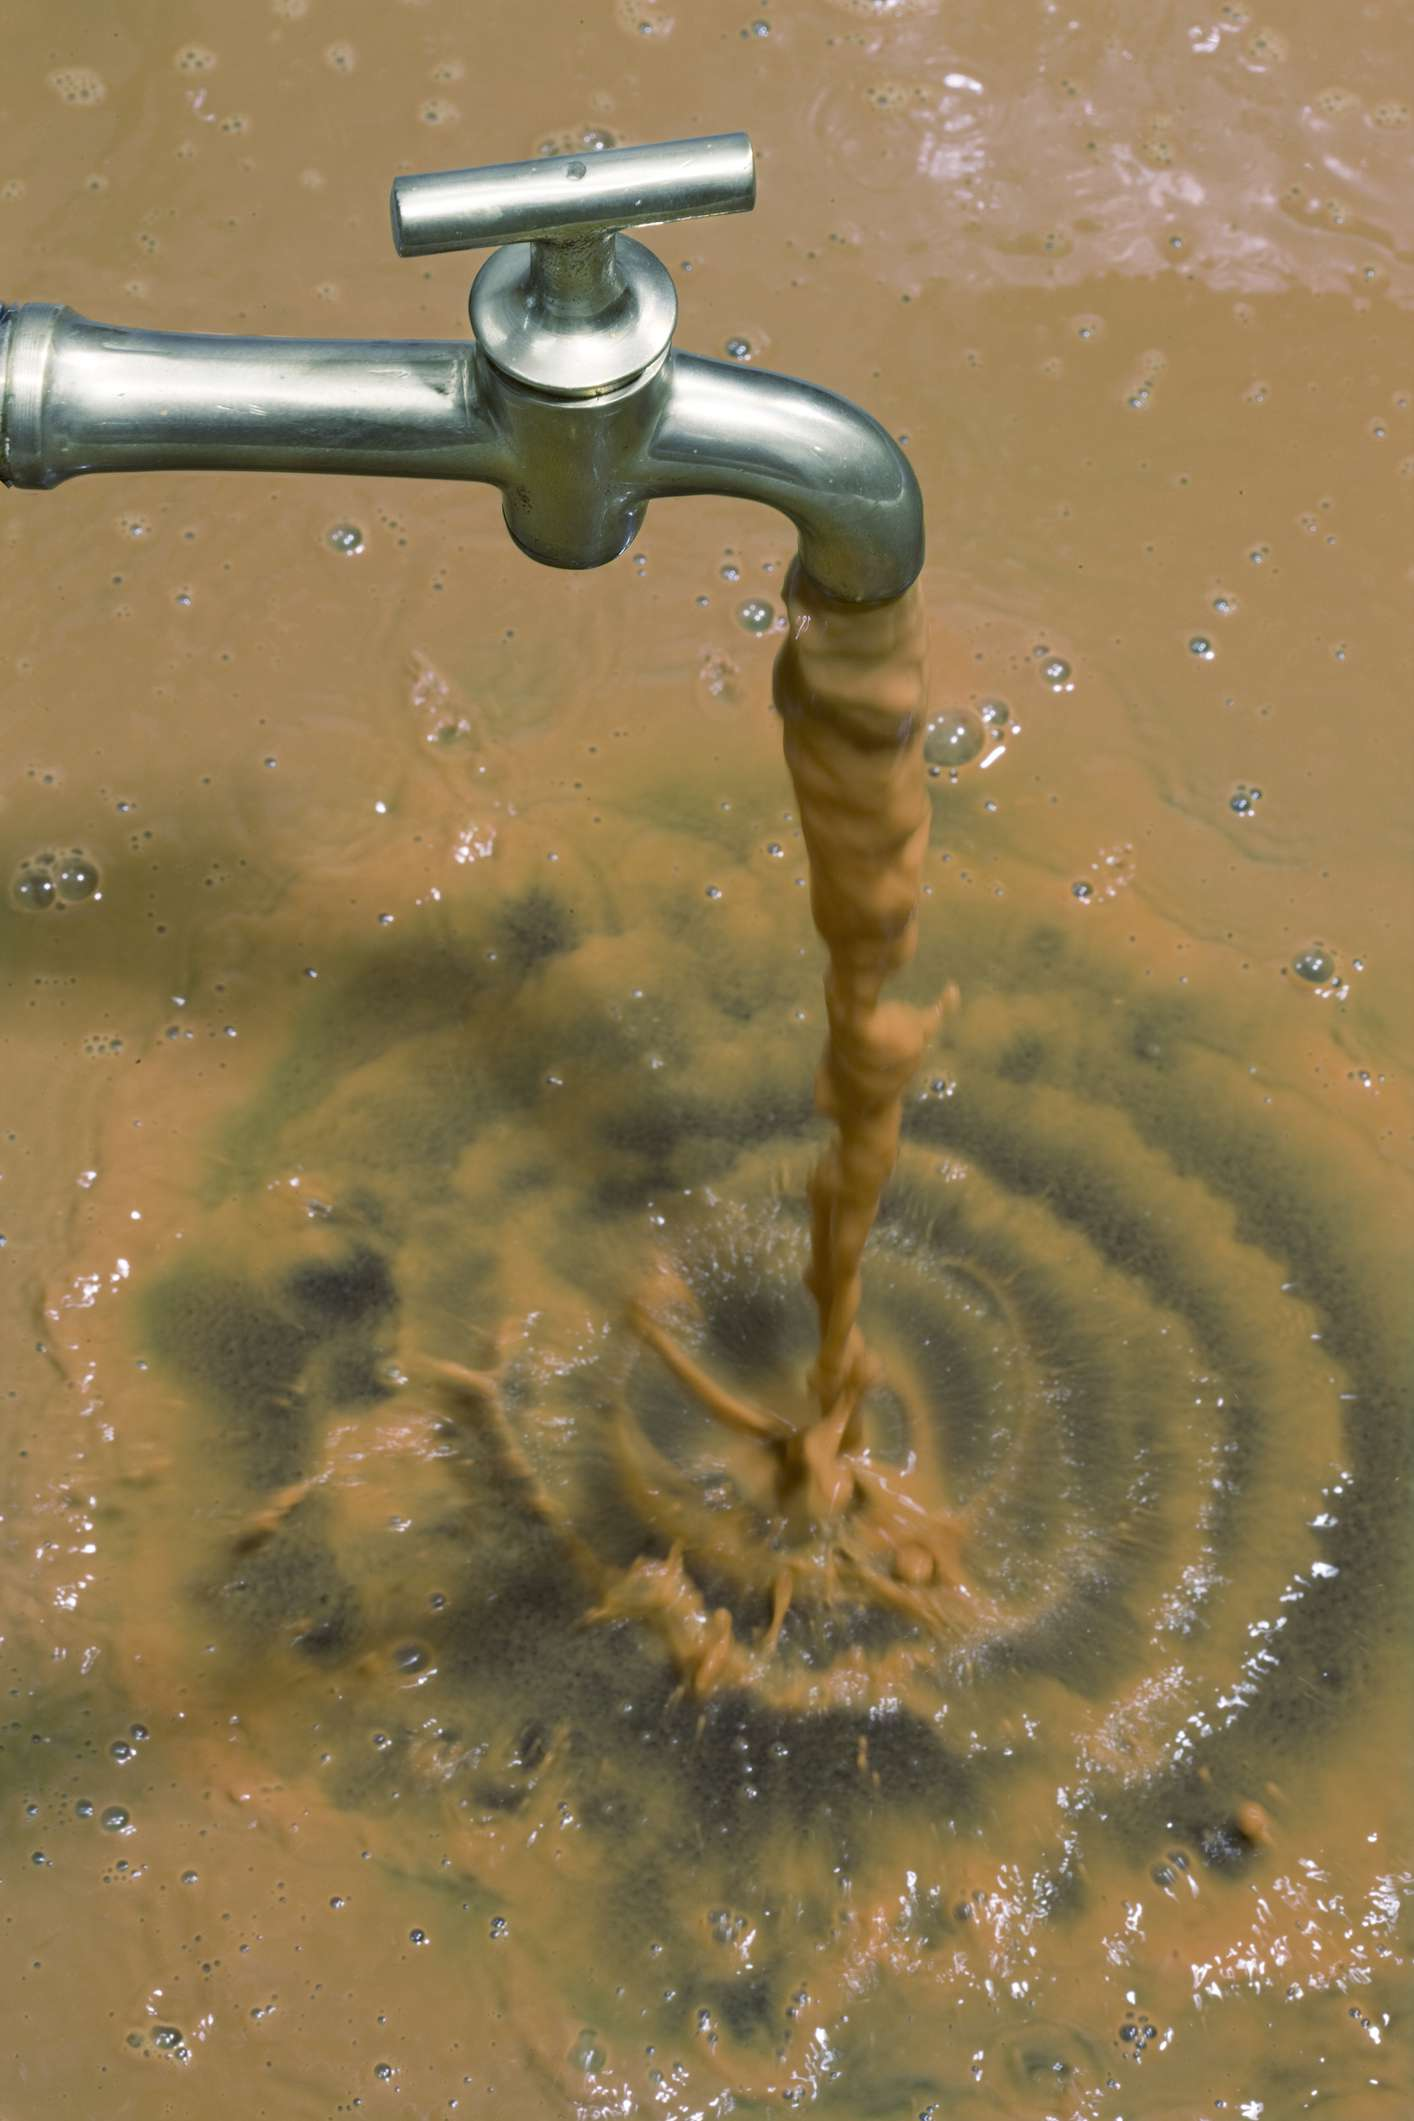
\includegraphics[width=0.9\textwidth]{figures/dirty2.jpg}
% \caption{Sample dirtyater.}
% \label{sample}
% \end{figure}

\subsection{Objectives}
The main objectives of this thesis is given below:
% to develop a system in which the water quality can be measured automatically and send those data to cloud server. Analysing water data many process like pumping water, sending alert message to the owner, making an early alarm can be done. Using Android application, the quality parameter can be downloaded. Even using secret account and browser, this database can be accessed. This smart system can be applied for water tank. By using this system fresh water can be supplied.
\begin{itemize}
    \item To make water quality monitoring system automated and better than all the past systems.
    \item To make the water quality monitoring system easier to WASA as well as people.
    \item To make the water tank cleaned thus in real life tank cleaning procedure is troublesome.
    \item To inform the person in charge about water quality.
    \item To supply fresh water to user.
\end{itemize}
 

% This system has features that are given below:
% \begin{itemize}
%     \item 

% \item This system can automatically pump water when the tank gets empty.
% \item This system can collect the pH level of water.
% \item This system can collect dirt level of water.
% \item This system can read the water temperature.
% \item This system can read the water temperature.
% \item It can analyze data and find that water is drinkable or not.
% \item It can make an early alarm when the water is contaminated.
% \item It can clean the water tank and can automatically flush water.
% \item It can send tank location to the person in charge.
% \end{itemize}

\section{Contribution of the Thesis}
The contributions of this thesis are given below:
\begin{itemize}
\item To calculate daily consumed water in real-time.
\item If water pollution occurs, send a warning message with location to the owner using GSM and GPS module.
\item Clean and flush the water tank automatically if the water quality goes dirty by analysing water data.
\end{itemize}

\section{Thesis Organization}
This paper has five chapters.
In chapter 1 describes some introductory description, design framework, application, motivation, history, implementation difficulties and contributions of the proposed system.
Chapter 2 gives an overview of the literature review and hardware component description, implementation challenges about this proposed system.
Chapter 3 discusses the system architecture, methodology, hardware components role, software components role and android application regarding this system.
Chapter 4 describes the experimental results, impacts and performance evaluation of the system.
Chapter 5 presents the conclusions, limitations and future recommendation regarding this.

\section{Conclusion}
In this chapter, a survey on water quality monitoring system based on IoT is written. Along with the problems, this chapter also describes the necessity of the water quality monitoring and controlling system. The inspiration and the contributions behind this work are also given here. The following chapter provides the context and current state of the issue.

